\section{Bottom-up block failure modeling}
\label{sec:bottom-up-modeling}
%TODO: Introduction

\subsection{Block failure characterization and modeling method}
\label{sec:block-failure-cz}

% What is bottom up
In a bottom-up approach, the study focuses first on the small-scale components of a system.
They are characterized individually, and a model is derived for each component.
Afterwards, these models are assembled together to match the full system architecture.
The main idea of a bottom-up approach is that a system is the sum of its parts.
Ultimately, we study if the robustness of a system can be assimilated as the sum of the robustness of its parts.
%TODO: Detail more

% Applicability to IC design
This approach fits well with the \gls{asic} design flow in general.
At some point in the design flow, the architecture of the integrated circuit is decided.
Then, each top-level function is split recursively into unit functions to be designed, to simplify the problem.
This part is rather a divide-and-conquer method, where a complex problem is split up into multiple simpler tasks.

Then, the design phase starts. It is a bottom-up method.
Transistors are assembled together to perform (usually one) unit function into what is called a \gls{block}.
Those blocks are then assembled together to build the more complex and interesting functionnalities.

% Why bottom up
The main perk of this characterization method is the inherent modularity.
The objective is to study each block independently of the others.
This way, the model built for each block is reusable.
A characterized block can be reused multiple times without having to do the characterization again each time.

% How is it done, core concept
The method described in this section starts by characterizing each block in a particular setup.
This setup provides appropriate biasing to the block, in order to set it in normal operating conditions.
This setup is also in charge of injecting the characterization signal on the tested input, and monitoring of the output under test.
Fig. \ref{block_function_cz} gives an example of such a characterization setup for a supply input.

%TODO: Improve figure (text sizes)
%TODO: Remove range comparator
\begin{figure}[!h]
  \centering
  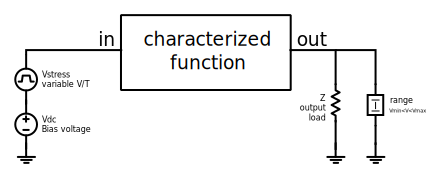
\includegraphics{src/4/figures/characterization_setup.pdf}
  \caption{Block characterization setup (supply input)}
  \label{block_function_cz}
\end{figure}

% What are the characterization signal
The characterization signal is a square waveform, applied on the tested input.
A set of simulations is ran with this setup.
Each simulation runs with a different pair of values for the \textbf{amplitude} and \textbf{duration} of the square signal.
Table \ref{parameterized-simulations} illustrates this simulation process.
Such testing method is called Wunsch and Bell in the litterature (REFERENCE).

\begin{table}[!h]
\centering
\begin{tabular}{@{}lllll@{}}
\toprule
    & 1ns   & 10ns  & 100ns & 1\textmugreek{}s   \\ \midrule
5V  & sim11 & sim21 & sim31 & sim41 \\
10V & sim12 & sim22 & sim32 & sim42 \\
15V & sim13 & sim23 & sim33 & sim43 \\ \bottomrule
\end{tabular}
\caption{Parameterized simulation planning for the characterization}
\label{parameterized-simulations}
\end{table}

In the time domain, this set of simulations is illustrated in Fig. \ref{set_input_signals}.

%TODO: Fix sim 12 sim12
\begin{figure}[!h]
  \centering
  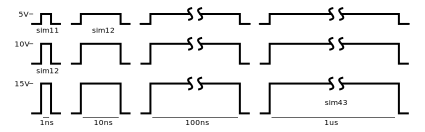
\includegraphics{src/4/figures/time_domain_cz_curves.pdf}
  \caption{Variations on (amplitude, duration) of the input characterization signal}
  \label{set_input_signals}
\end{figure}

% What is the direct result of the characterization, how to obtain it
For each simulation, the waveform of the output under test is recorded.
The waveform is compared against a threshold.
This threshold can also be seen as failure criteria of the studied function.
%TODO: Donner un example : If we consider the pre-reg block, the failure criteria will be ...

This treshold is set prior to the simulation.
There is no general rule for setting it.
The \gls{dc} specification of the output can be used directly, if it exists, or a sound value in regard of the design, or an arbitrary level.

If the waveform goes above (maximum threshold) or below (minimum threshold), the simulation is marked as \textit{fail}.
For each simulation, the duration during which the failure criteria was violated is also recorded.
Once all simulations are complete, it is known which ones contain a \textit{fail}.

The results are summarized into table \ref{simulation-results}.

\begin{table}[!h]
\centering
\begin{tabular}{@{}lllll@{}}
\toprule
    & 1ns                          & 10ns                         & 100ns                        & 1\textmugreek{}s             \\ \midrule
5V  & {\color[HTML]{32CB00} sim11} & {\color[HTML]{32CB00} sim21} & {\color[HTML]{32CB00} sim31} & {\color[HTML]{FE0000} sim41} \\
10V & {\color[HTML]{32CB00} sim12} & {\color[HTML]{FE0000} sim22} & {\color[HTML]{FE0000} sim32} & {\color[HTML]{FE0000} sim42} \\
15V & {\color[HTML]{FE0000} sim13} & {\color[HTML]{FE0000} sim23} & {\color[HTML]{FE0000} sim33} & {\color[HTML]{FE0000} sim43} \\ \bottomrule
\end{tabular}
\caption{Example of results on a set of simulations (simulations in red contain a fail)}
\label{simulation-results}
\end{table}

% A first visualization of the characterization
A curve can be build from this table, to make visualization easier.
It gives a visual representation of the functionnal robustness of the block.
Following table \ref{simulation-results}, the x axis is the duration of the input stress.
The y axis is the amplitude of the input signal during the stress.
This amplitude is the voltage or current seen by the characterized input pin.
It is the sum of the stress amplitude and an eventual biasing level.
Finally, each point (x,y) of the curve represents the \textbf{minimal} amplitude (y) for the given pulse width (x) at which failures occur.

Fig. \ref{wb_cz_curve_example} gives an example of such a characterization curve.

%TODO: REVOIR COULEURS
\begin{figure}[!h]
  \centering
  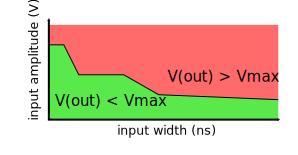
\includegraphics{src/4/figures/example_curve.pdf}
  \caption{Principle of Wunsch and Bell curve for powered-on block testing}
  \label{wb_cz_curve_example}
\end{figure}

% How to improve the displayed information
The duration during which an output is in fail was recorded for each simulation, as stated earlier.
% WHY IS THIS IMPORTANT
It is possible to improve table \ref{simulation-results} by replacing the \textit{fail} by the duration of the fail.
This is illustrated in table \ref{simulation-results-bis}.

\begin{table}[!h]
\centering
\begin{tabular}{@{}lcccc@{}}
\toprule
    & \multicolumn{1}{l}{1ns}      & \multicolumn{1}{l}{10ns}     & \multicolumn{1}{l}{100ns}    & \multicolumn{1}{l}{1us}     \\ \midrule
5V  & {\color[HTML]{32CB00} }      & {\color[HTML]{32CB00} }      & {\color[HTML]{32CB00} }      & {\color[HTML]{F56B00} 2us}  \\
10V & {\color[HTML]{32CB00} }      & {\color[HTML]{00D2CB} 125ns} & {\color[HTML]{F8A102} 540ns} & {\color[HTML]{FE0000} 30us} \\
15V & {\color[HTML]{00D2CB} 110ns} & {\color[HTML]{FFCB2F} 150ns} & {\color[HTML]{FE0000} 30us}  & {\color[HTML]{FE0000} 30us} \\ \bottomrule
\end{tabular}
\caption{A more informative representation of all simulation results to account for duration of output failure}
\label{simulation-results-bis}
\end{table}

% How to improve the curve from the improved table
This improvement can also be transfered to the curve representation.
A gradient can be used rather than a simple failure curve.
For each point of the curve, the gradient will have a value representing the duration of the failure on \textbf{\textit{V(out)}}.
The figure \ref{wb_cz_curve_example_v2} provides an example of this improved representation.
In this figure, the warmer the gradient, the longer the output is disturbed.

\begin{figure}[!h]
  \centering
  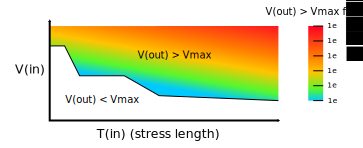
\includegraphics{src/4/figures/example_curve_v2.pdf}
  \caption{Improved curve for Wunsch and Bell powered-on characterization}
  \label{wb_cz_curve_example_v2}
\end{figure}

The gradient can also be discretized into a few aeras for better readability as shown in figure \ref{wb_cz_curve_example_v2_discrete}.
This representation looses some information compared to the gradient one, but is easier to generate and read.
This is the representation we have adopted further in this study, to express the functionnal robustness of a single block.

\begin{figure}[!h]
  \centering
  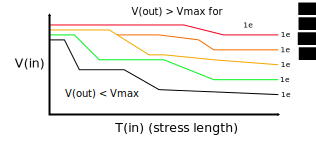
\includegraphics{src/4/figures/example_curve_v2_discrete.pdf}
  \caption{Improved discrete curve for Wunsch and Bell powered-on characterization}
  \label{wb_cz_curve_example_v2_discrete}
\end{figure}

%TODO: Comment this figure
\begin{figure}[!h]
  \centering
  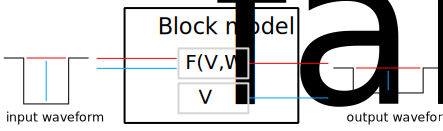
\includegraphics{src/4/figures/principle_transfert_function.pdf}
  \caption{First modelling method}
  \label{fig:principle-transfert-func}
\end{figure}


\subsection{Block models chaining}
\label{sec:block-chaining}

% Explain the chaining mechanism
The characterization process detailed previously (in \ref{sec:block-failure-cz}) is repeated on each block constituting a high-level function.
Once done, the bottom-up study now focuses on a higher level in the design hierarchy.
As a remainder, the original goal of this method is to see if the robustness of a high-level function is the sum of its parts' robustness.

Thus, individual models are connected together, by following exactly how blocks are connected in the design.
To illustrate this idea, fig. \ref{example_toplevel_function} represents an example of a high-level function, constituted of three blocks at the second level of hierarchy.
It is assumed that each of these blocks has been characterized.

% WHICH NET IS TOP MONITORED ?

\begin{figure}[!h]
  \centering
  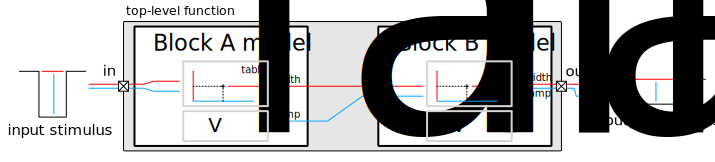
\includegraphics{src/4/figures/example_top_level_function.pdf}
  \caption{Example of a top-level function with 3 characterized blocks}
  \label{example_toplevel_function}
\end{figure}

% Remind the final goal
Now, we want to obtain the robustness of the entire function, against a given stress, using the block models.
The stress is injected on the global pin \textbf{\textit{in}}.

% What is the input stress ? What is the top-level function evaluated against ?
In this example, we will consider the stress is generated by a \gls{tlp} generator, and is thus rectangular.
For this example, the stress is chosen to have a duration of 100 ns, and an amplitude of 10V.
Section \ref{sec:wb-for-arbitrary-wvfs} describes methods for applying the block models to arbitrary input waveforms.

% How is used the characterization of the output of A on the input of B ?
%TODO: Detail a lot more. This is key. Speak about modeling of the output, and simplification to square pulse.
%TODO: Make a figure to show how is the disturbance on the output of A is modeled
The stress is injected on the global \textbf{\textit{in}} pin.
This pin is also the input pin of the first block.
Thus, the properties of the \gls{tlp} pulse can directly be applied to the model of block A.
Fig. \ref{example_complete_curve} shows an example curve for model A, and the location of the TLP pulse characteristics on this curve.


\begin{figure}[!h]
  \centering
  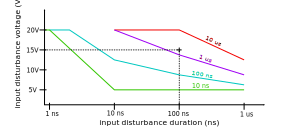
\includegraphics{src/4/figures/example_complete_curve.pdf}
  \caption{Model A curve and determination of impact of the TLP pulse - values in color represent the duration of failure on the output}
  \label{example_complete_curve}
\end{figure}

% Interpretate stress to deduce net1
Like stated earlier, the pulse has a duration of 100ns and an amplitude of 15V. By reporting this point on curve \ref{example_complete_curve},
it is visible that this will cause the output of block A to violate its failure criteria between 1 \textmugreek{}s and 10 \textmugreek{}s.
We consider, for the sake of this example, the failure criteria of block A to be net1 > 5V.
With a 100ns long 15V pulse on the input of A, the characterization states that the output of block A will go above 5V for at least 1us.
This is the best case value for net1.

% Use net1 as input of next block
\textit{net1} is the output of block A, but it is also the input of block B.
Thus, best case (amplitude, duration) values for net1 can be used as input for block B's model.
Fig. \ref{example_complete_curve_B} shows an example curve for model B, and the location of the \textit{net1} disturbance on this curve.
This shows that \textit{net2}, the output of block B and the input of block C, will go below B's failure level for at least 10 \textmugreek{}s.

\begin{figure}[!h]
  \centering
  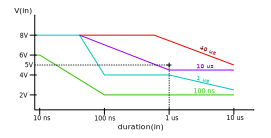
\includegraphics{src/4/figures/example_complete_curve_B.pdf}
  \caption{Model B curve and determination of impact of the TLP pulse}
  \label{example_complete_curve_B}
\end{figure}

% Repeatable process
As shown, this process can be repeated in theory with as many blocks as required by the original design, until the final pin is reached.
The is possible because the output of a block is used as the input of the next one.

%TODO: Algorithm organigram

% How to select pins to characterize

% Show how it can help to speedup and simplify the computation of the entire function robustness
